\section{Statistics}


%%%%%%%%%%%%%%%%%%%%%%%%%%%
%
% Probability Distributions
%
%%%%%%%%%%%%%%%%%%%%%%%%%%%

\formdesc{Expected Value}

\begin{equation}
	E(X) = \mu = \sum_{i=1}^k x_i ~ P(X = x_i)
\end{equation}

for a discrete random variable with $k$ possible values.
\hformbar




\formdesc{General Variance Formula}

\begin{equation}
	Var(X) = \sigma^2 = \sum_{j=1}^k (x_j - \mu)^2 ~ P(X = x_j),
\end{equation}

or, the sum of the squared deviations $(x_j - \mu)^2$ weighted by the corresponding probabilities $P(X=x_1),  \ldots, P(X=x_k)$.
\hformbar



\formdesc{General Standard Deviation}

\begin{equation}
	\sigma = \sqrt{\sigma^2} = \sqrt{Var(X)}
\end{equation}
\hformbar



\formdesc{Linear Combinations of Variables}

\begin{equation}
	Z = aX + bY
\end{equation}

is a linear combination of the independent, random variables $X$ and $Y$ (often $a$ and $b$ are $1$ or $-1$). 

\begin{eqnarray}
  E(Z) &=& a \times E(X) + b \times E(Y) \\
  Var(Z) &=& a^2 \times Var(X) + b^2 \times Var(Y)
\end{eqnarray}
\hformbar



\formdesc{Probability Density Function (PDF)}

\begin{equation}
	P(a \leq X \leq b) = \int_{a}^{b} f(x) ~ dx
\end{equation}


is a PDF of $X$, for any two numbers $a$ and $b$ where $a \leq b$. I.e., the probability that $X$ takes on a value in the interval $[a, b]$ is the area above this interval and below the graph of the density curve.

\begin{itemize}
	\item $P(X=c) = 0$ for any constant (bins are infinitesimally small)
	\item $\sum P(x_i) = 1$
\end{itemize}


\hformbar



\formdesc{Normal Distribution v. Standard Normal}

There is any entire family of distributions that can be called normal, but the
prototypical distribution with mean of $0$ and standard deviation of $1$ is
called the standard normal. Formally defined by its PDF as:

\begin{equation}
  f(x \mid \mu, \sigma^2) = \frac{1}{\sqrt{2 \pi \sigma^2}} \, e^{ \frac{-(x - \mu)^2}{2 \sigma^2}}
\end{equation}

\subsection*{Properties}

\begin{enumerate}
	\item Symmetric around mean
	\item Mean = mode = median
	\item Denser at center than in tails
\end{enumerate}

Consequently,

\begin{itemize}
	\item 68 percent of distribution is within one standard deviation of the mean
	\item 95 percent of distribution is within approximately two standard deviations of the mean
\end{itemize}
\hformbar



\formdesc{Evaluating Normality}

\begin{center}
    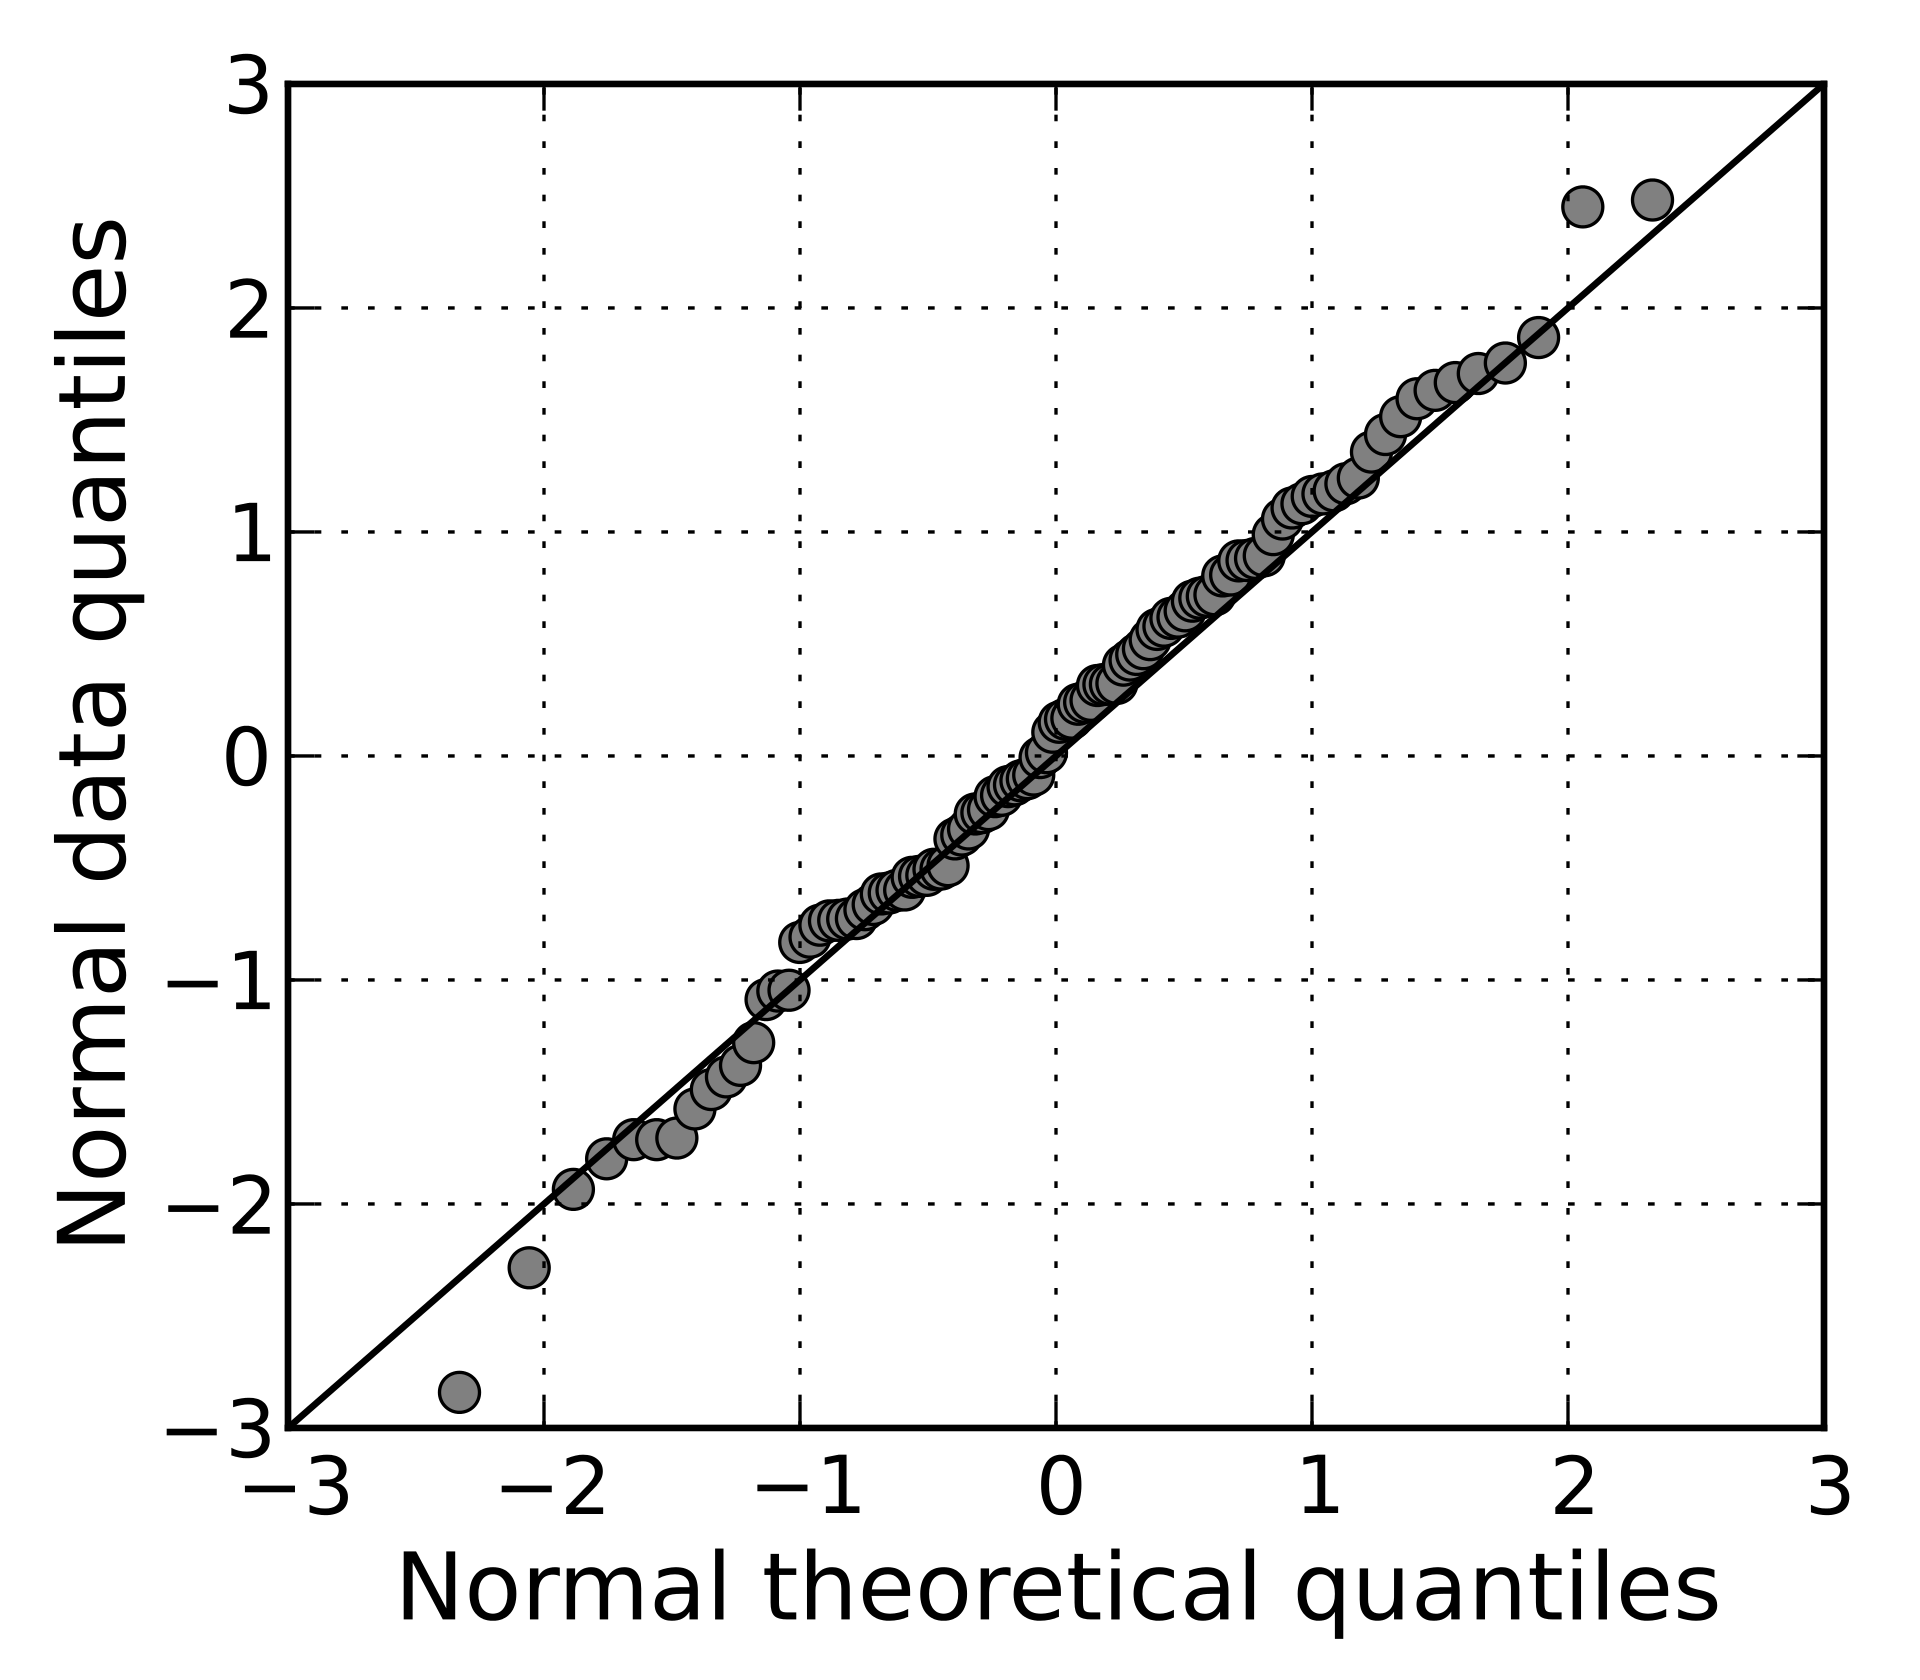
\includegraphics[width=1.5in]{normal_qq}
\end{center}

\begin{itemize}
	\item A normal probability plot using quartiles can be used to evaluate how closely a given distribution adheres to normality, where the straight line is a perfect normal curve
	\item As $N$ increases, the deviation from normality will decrease
\end{itemize}

\hformbar



\formdesc{Z Scores}

\begin{equation} Z = \frac{x - \mu}{\sigma}\end{equation}

converts any value from a normal distribution to its corresponding value on the standard normal distribution

\begin{itemize}
	\item Describes the number of standard deviations a point is from the mean $\mu$
	\item Z scores to the left of $\mu$ are negative, and positive to the right of $\mu$
\end{itemize}
\hformbar



\formdesc{Z Scores: Probabilities on Normal Distribution}

\subsection*{Ex. What is the probability $X > A$, given $X \sim N(\mu=1500, \sigma=300)$?}

\begin{equation}
	Z = \frac{x - \mu}{\sigma} = \frac{1630 - 1500}{300} = 0.43
\end{equation}

This is 0.6664 on Z table, so 66.64 percent of $X$ is to the left of A so:

\begin{equation}
	1 - 0.6664 = 0.3336
\end{equation}

The probability $X > A$ is 33.36 percent.


\subsection*{Ex. Given $A = 1400$ and $X \sim N(\mu=1500, \sigma=300)$, what is the percentile corresponding to A?}

\begin{equation}
	Z = \frac{x - \mu}{\sigma} = \frac{1400 - 1500}{300} = -0.33
\end{equation}

The corresponding value on the Z table is 0.3707, so $A$ is the 37th percentile.


\subsection*{Ex. Given $p = .40$ and $X \sim N(\mu=70, \sigma=3.3)$, what is the value corresponding to percentile $p$?}

Lookup $p$ on Z table, getting a $Z = -0.25$. Work backwards:

\begin{equation}
	-0.25 = Z = \frac{x - \mu}{\sigma} = \frac{x - 70}{3.3}
\end{equation}

and solve for $x = 69.18$.


\subsection*{Ex. What is the probability $X$ is between $A$ and $B$, given $X \sim N(\mu, \sigma)$?}

Using Z-scores method, find the area to the left of $A$ and to the right of $B$, then $A - B = 1 -$ area left of $A -$ are to right of $B$.
\hformbar



\formdesc{Bernoulli Distribution}

\begin{equation}
	P(X = x) = \left\{\begin{matrix}
					  p ~$for$~ x = 1\\ 
                      1 - p ~$for$~ x =0
                \end{matrix}\right.
\end{equation}

describes the distribution of individual trials with two possible outcomes, success or failure, described by proportion of successes $0 \leq p \leq 1$:

\begin{eqnarray}
  \hat{p}   &=& \frac{\mid successes \mid}{\mid failures \mid} \\
  \mu       &=& p \\
  \sigma^2  &=& p(1 - p)
\end{eqnarray}

\begin{itemize}
	\item The probability of success after $n$ trials is $(1 - p)^{n - 1} \times p$
\end{itemize}

\hformbar



\formdesc{Bernoulli: Geometric Distribution}

\begin{center}
    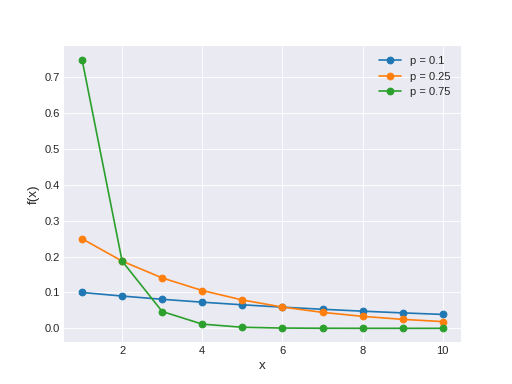
\includegraphics[width=2in]{geometric_dist}
\end{center}

describes the wait time until a success for \textit{independent} Bernoulli random variables; or, the probability of observing the $k$-th success by the $n$-th trial

\begin{eqnarray}
  \mu       &=& \frac{1}{p} \\
  \sigma^2  &=& \frac{1 - p}{p^2}
\end{eqnarray}

\begin{itemize}
	\item Higher $p$ means fewer trials until success
	\item Can never be approximated by a normal distribution
\end{itemize}

\hformbar



\formdesc{Binomial Distribution}

\begin{center}
    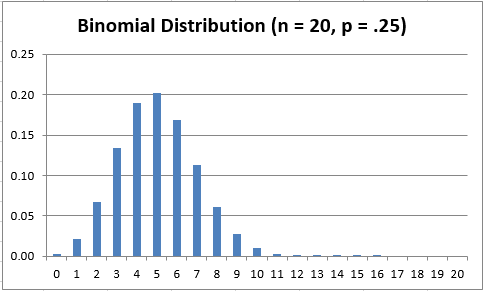
\includegraphics[width=2in]{binomial}
\end{center}

describes the probability of having exactly $k$ successes in $n$ independent Bernoulli trials (with probability of success $p$):

\begin{eqnarray}
	P(x = k \mid n, \mu, \sigma) &=& \begin{pmatrix}
		n\\ 
		k
	\end{pmatrix}
	p^k (1 - p)^{n -k} \\
	&=& \frac{n!}{k!(n - k)!} ~p^k (1 - p)^{n - k} 
\end{eqnarray}

Parameters, can be used to approximate to normal when $n$ is sufficiently large and $np$ and $n(1-p)$ are both greater than or equal to 10:

\begin{eqnarray}
  \mu       &=& np \\
  \sigma^2  &=& np(1 - p)
\end{eqnarray}

\hformbar



\formdesc{Poisson Distribution}

\begin{center}
    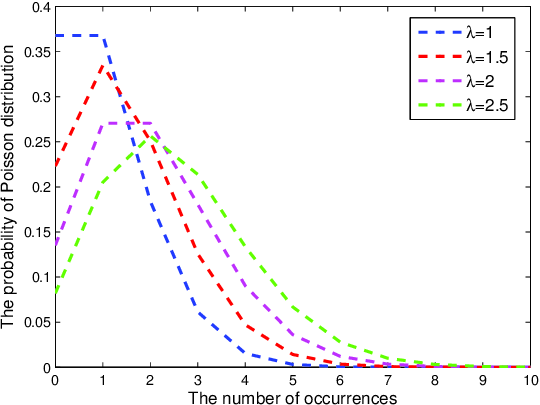
\includegraphics[width=2in]{poisson}
\end{center}

\begin{equation}
	P(X = x \mid \lambda) = \frac{\lambda^x e^{-\lambda}}{x!}
\end{equation}

Describes the number of events in a larger population over a unit of time with rate $\lambda$:

\begin{eqnarray}
  \mu       &=& \lambda \\
  \sigma^2  &=& \lambda
\end{eqnarray}

\hformbar







%%%%%%%%%%%%%%%%%%%%%%%%
%
% Inferential Statistics
%
%%%%%%%%%%%%%%%%%%%%%%%%























\formdesc{Inferential Statistics}

The body of thought governing the inferences of populations from samples,
and how these sample statistics can vary.
\hformbar



\formdesc{Standard Error}

\begin{equation}
	SE = \frac{\sigma}{\sqrt{n}}
\end{equation}

is the standard deviation of distributions of sample statistics, when population $\sigma$ is known. If it is unknown, and if $n > 30$, substitute sample standard deviation $s$

\begin{itemize}
	\item $SE$ decreases as $n$ increases
	\item $SE$ decreases as $\sigma$ (or $s$) decreases
\end{itemize}
\hformbar



\formdesc{Confidence Intervals}

\begin{equation}
	\bar{x} \pm z \times SE
\end{equation}

\begin{itemize}
	\item $\bar{x}$ is the sample statistic, such as sample mean
	\item $z \times SE$ is the \textit{margin of error}
	\item $z$ is the desired confidence level, e.g., $z = 1.96$ for a 95 percent confidence interval
\end{itemize}

\textit{Interpretation.} ``We are $Z$ percent confident the true population \textit{statistic} is between $A$ and $B$''; or, ``$Z$ percent of samples will have a \textit{sample statistic} between $A$ and $B$.''

\hformbar



\formdesc{Central Limit Theorem}

Given a population with a finite mean $\mu$ and a finite non-zero variance
$\sigma^2$, the sampling distribution of the mean approaches a normal
distribution with a mean of $\mu$ and a variance of $\frac{\sigma^2}{N}$, as
$N$, the sample size, increases---regardless of the shape of the parent population.
\hformbar




\formdesc{Hypothesis Testing}

\begin{table}[]
\begin{tabular}{ll}
One-Sided      & Two-Sided       \\
$H_0: x = A$   & $H_0: x = A$    \\
$H_A: x >/< A$ & $H_A: x \neq A$
\end{tabular}
\end{table}

The process of comparing two point estimates, to determine if any difference between them is ``real'' or the result of natural variance in samples.

\begin{itemize}
	\item \textit{Type I} errors, or false positives, occur when the null hypothesis  is true, but rejected
	\item \textit{Type II} errors, or false negatives, occur when the alternative hypothesis is true, and the null hypothesis is not rejected
\end{itemize}

\subsection*{Quantifying Risk}

\begin{itemize}
	\item The risk of Type I errors is quantified by $\alpha$, i.e., the probability the point estimate is more than $z^*$ standard deviations away from the true population parameter
	\item The $p$-value is $1 - \alpha$, the probability of observing data at least as favorable to the alternative hypothesis as the present data set, if the null hypothesis is true
\end{itemize}

\subsection*{One- and Two-Sided Hypotheses}

% Move to top, use a table with 2 columns and 3 rows, as in notes



\hformbar










%%%%%%%%
%
% Trash?
%
%%%%%%%%


\formdesc{Sample Statistics: Mean and Variance}

\begin{itemize}
  \item $\mu_M = \mu$ is the mean of the sampling distribution of means
  \item $\sigma_M^2 = \frac{\sigma^2}{N}$ is the variance of the sampling
	distribution of the mean
  \item $\sigma_M = \frac{\sigma}{\sqrt{N}}$ is the standard error of the sampling
	distribution of the mean
\end{itemize}

As $N$ increases, variance of sample mean decreases
\hformbar




\formdesc{Sample Statistics: Difference in Mean}

Two samples from a population the size $n_1$ and $n_2$, calculate the means
$M_1$ and $M_2$, and the difference is $M_1 - M_2$

\begin{eqnarray}
  \mu_{M_1 - M_2} &=& M_1 - M_2 \\
  \sigma_{M_1 - M_2}^2 &=& \sigma_{M_1}^2 + \sigma_{M_2}^2 \\
  \sigma_{M_1 - M_2} &=& \sqrt{\frac{\sigma_1^2}{n_1} + \frac{\sigma_2^2}{n_2}}
\end{eqnarray}

When variance and sample size are the same, standard error becomes:

\begin{equation}
  \sigma_{M_1 - M_2} = \sqrt{\frac{\sigma_1^2}{n_1} + \frac{\sigma_2^2}{n_2}}i
  = \sqrt{ \frac{\sigma^2}{n} + \frac{\sigma^2}{n}}
  = \sqrt{ \frac{2 \sigma^2}{n} }
\end{equation}

If $n_1 \neq n_2$ then variance becomes:

\begin{equation}
  \sigma_{M_1 - M2}^2 = \frac{\sigma_1^2}{n_1} + \frac{\sigma_2^2}{n_2}
\end{equation}

\subsection*{What is the probability that the mean of sample 1 will exceed that of
sample 2 by $N$ or more?}

\begin{enumerate}
  \item Find mean: $\mu_{M_1 - M_2} = M_1 - M_2$
  \item Find standard error: $\sigma_{M_1 - M_2}$
  \item Find area underneath distribution of sample 1 to the right of the mean
	of sample 2 plus $N$
\end{enumerate}

\hformbar



\formdesc{Sample Statistics: $r$ and $\rho$}

\begin{itemize}
  \item Not normally distributed---right-skewed---because correlation cannot
	exceed 1
  \item As $\rho$ increases, the more right-skewed the distribution
\end{itemize}

\hformbar



\formdesc{Sample Statistics: Proportion $\pi$}

Sampling proportion is closely related to the binomial distribution---the
total number of successes---where $p$ is the distribution of the mean number of
successes

\begin{eqnarray}
  \mu_p &=& \pi \\
  \sigma_p &=& \frac{\sqrt{N \pi (1 - \pi)}}{N}
           = \sqrt{\frac{\pi (1 - \pi)}{N}}
\end{eqnarray}

\subsection*{Find probability $p$ is greater than $A$}

Given $N$ and population proportion $\pi$:

\begin{enumerate}
  \item Find mean of $p = \pi$
  \item Calculate standard error as above
  \item Conduct as normal distribution given $N$ is sufficently large and $\pi$
	is not too close to 0 or 1
\end{enumerate}

\hformbar



\formdesc{Estimation}

The process of estimating population parameters from sample statistics. Usually
results in a point estimate as well as interval estimates called confidence
intervals.

\hformbar



\formdesc{Degrees of Freedom}



\hformbar

\subsection{Chapter 3 questions}

What percent of the standard normal distribution is found in Z >/< A? A: Use pnorm() or a Z table. If A is negative and we want to know Z > A, we know the percent is greater than 15. If |Z| < 0.5 -- the bounds are -.5 and 0.5, so Z(.5) - Z(-.5).

Normal distributions described as $m ~ N(\mu, \sigma)$.

Problem 3.4. Given two distributions, and two points in each, which does each compare relative to their groups? 1. Convert both points into Z scores, and compare them. You can also convert the Z-scores into probabilities to say the percent they beat/were beaten by.

Geometric examples: \url{https://www.redbrick.dcu.ie/~minisham/CA/Notes/CA266/10_Geometric_Distribution.pdf}

Problem No. 3.18. 68-95-99.7\% rule.

Problem No. 3.22. Given a probability distribution of a sequence, what is the probability the Xth item meets some condition (number of coin tosses til heads, number of products produced until defect, etc.)? Use geometric distribution.

Problem No. 3.22.d. What is the probability the sequence produces no defects after n? Uses factorials

Problem No. 3.22.c. How many in the sequence before the first defect? This is mean or expected value of geometric distribution.

Problem No. 3.38. Binomial model to calculate 2/3 kids will be boys.

Problem No. 3.42. Probability on the Nth trial will have the Mth success? Solved similar as above with binomial model? Referring to a probability distribution, not a discrete event (like gambler's fallacy).



\subsection{Chapter 4 Questions}

Problem No. 4.4e. Measure uncertainty around a point estimate by computing a 95\% confidence interval


\newpage
